\section{Hovdyr (Artsbestemmelse, biologi \& terminologi)}

% ========== TITEL: HOVDYR ==========
\begin{frame}
  \vspace{1.5em}
  \begin{center}
    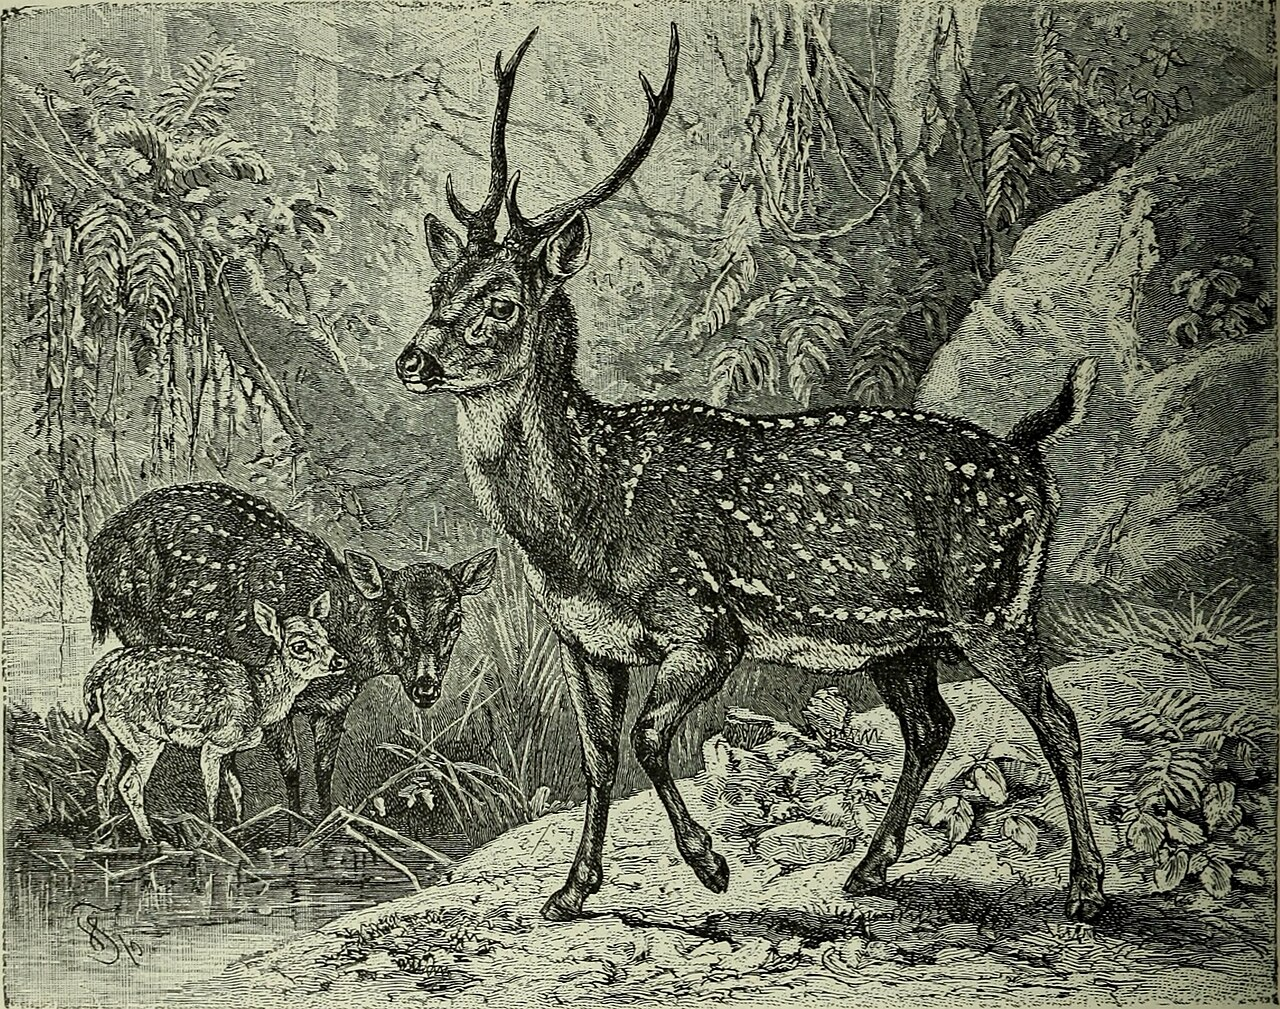
\includegraphics[width=12cm, height=4cm, keepaspectratio]{Billeder/Dyr/Pattedyr/hovdyr/hovdyr.jpg}\\[1.2em]
    {\LARGE \textbf{Hovdyr}}\\[0.6em]
    Klovbærende vildt\\[0.35em]
    Artsbestemmelse, vildtbiologi \& terminologi \\[0.9em]
    {\tiny\color{gray}
    CC BY 4.0 – kan frit anvendes, også kommercielt. Rettighederne må ikke skærpes.\\[0.05em]
    Udviklet af Aleksander Sønder, OSJAGTTEGN.DK}
  \end{center}
\end{frame}

% ========== KRONHJORT (KRONVILDT) ==========
\begin{frame}{%
  \begin{minipage}[c]{0.30\textwidth}
    Kronhjort
  \end{minipage}%
  \hfill
  \begin{minipage}[c]{0.45\textwidth}
    \footnotesize
    \textbf{Jagttid:} $\geq$ 10 sprosser: 16.\ okt.--31.\ dec.\\
    %Spids: 1.\ sep.--31.\ jan.\ \ Hind: 1.\ okt.--31.\ jan.\\
    %Kalv: 1.\ sep.--29.\ feb.*
  \end{minipage}%
  \hfill
  \begin{minipage}[c]{0.15\textwidth}
    \noindent\raggedleft
    
\includegraphics[width=0.5cm, height=0.5cm, keepaspectratio]{Billeder/Ikoner/star.png}%
    \hspace{0.2em}%
    
\includegraphics[width=0.5cm, height=0.5cm, keepaspectratio]{Billeder/Ikoner/star.png}%
    \hspace{0.2em}%
    
\includegraphics[width=0.5cm, height=0.5cm, keepaspectratio]{Billeder/Ikoner/star.png}
  \end{minipage}%
}
  \vspace{0.25em}
  \begin{columns}[T]
    % --- Venstre kolonne: Tekst ---
    \column{0.45\textwidth}
    \setlength{\parskip}{0.4em}
    \tiny
    \RaggedRight
    \textbf{\textit{Cervus elaphus}} – største hjorteart i Danmark. Hannen kaldes kronhjort og kendes på det store, forgrenede gevir. I andet leveår kaldes den kronspidshjort. \par
    \textbf{Udseende:}\\
    \quad – Langt snudeskaft \\
    \quad – Gult spejl der går op på ryggen \\
    \quad – Lange ører \par
    \textbf{Levesteder:} Store skovområder. Kræver meget ro. Nataktiv og opholder sig i tæt vegetation om dagen. \par
    \textbf{Føde:} Lyng, græs, lav, landbrugsafgrøder, skud fra buske/træer. \par
    \textbf{Udbredelse:} Jylland og Sjælland. \par
    \textbf{Parring/brunst:} September/oktober. \par
    \textbf{Forplantning:}\\
    \quad – \textbf{Kønsmoden:} 1 år \\
    \quad – \textbf{Mono/polygam:} Polygam \\
    \quad – \textbf{Bestandsomsætning:} Langsom \\
    %\quad – \textbf{Kuld:} 1 kalv, sjældent 2 \par
    %\textbf{*Bemærk:} Mange lokale jagttider.
    % --- Højre kolonne: Større billede ---
    \column{0.52\textwidth}
    \centering
    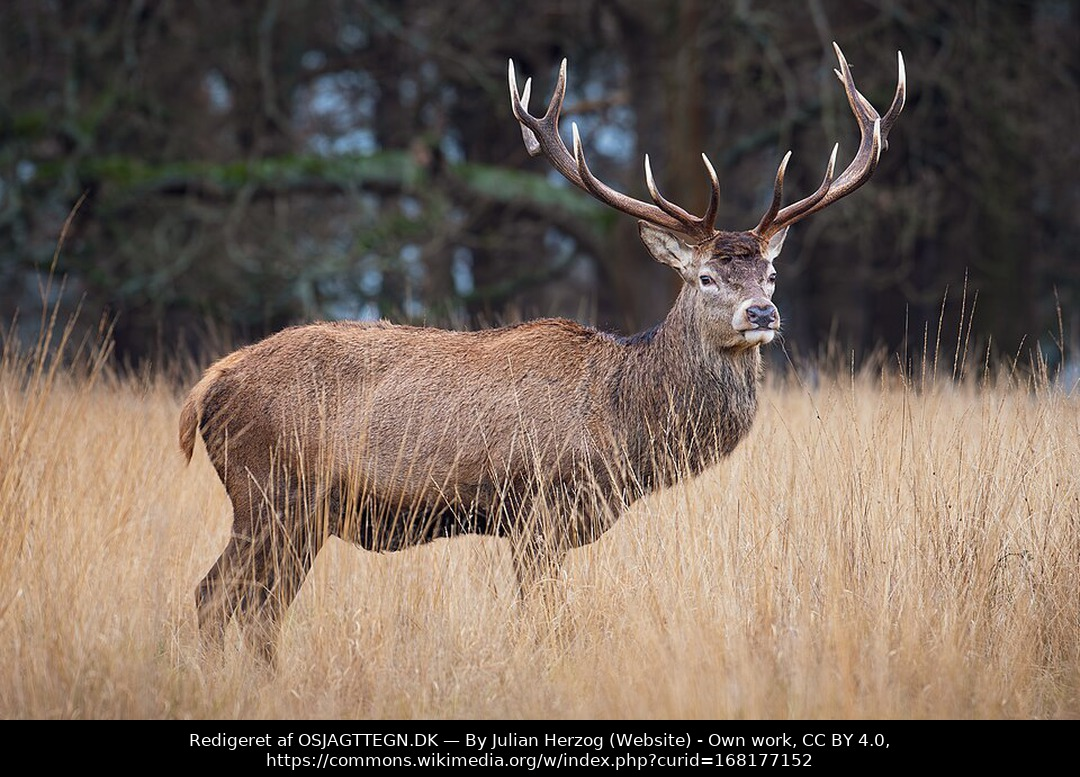
\includegraphics[width=\linewidth, height=7.2cm, keepaspectratio]{Billeder/Dyr/Pattedyr/hovdyr/kronvildt/kronhjort/kronvildt-male-03.jpg}
  \end{columns}
\end{frame}

% ========== KRONSPIDSHJORT ==========
\begin{frame}{%
  \begin{minipage}[c]{0.30\textwidth}
    Kronspidshjort
  \end{minipage}%
  \hfill
  \begin{minipage}[c]{0.45\textwidth}
    \footnotesize
    \textbf{Jagttid:} 1.\ september -- 31.\ januar
  \end{minipage}%
  \hfill
  \begin{minipage}[c]{0.15\textwidth}
    \noindent\raggedleft
    
\includegraphics[width=0.5cm, height=0.5cm, keepaspectratio]{Billeder/Ikoner/star.png}%
    \hspace{0.2em}%
    
\includegraphics[width=0.5cm, height=0.5cm, keepaspectratio]{Billeder/Ikoner/star.png}%
    \hspace{0.2em}%
    
\includegraphics[width=0.5cm, height=0.5cm, keepaspectratio]{Billeder/Ikoner/star.png}
  \end{minipage}%
}
  \vspace{0.25em}
  \begin{columns}[T]
    % --- Venstre kolonne: Tekst ---
    \column{0.45\textwidth}
    \setlength{\parskip}{0.4em}
    \tiny
    \RaggedRight
    \textbf{\textit{Cervus elaphus}} – kronhjort i sit andet leveår. Kaldes spidshjort, fordi geviret typisk kun består af to enkelte spidser. \par
    \textbf{Udseende:}\\
    \quad – To enkle gevirstænger uden forgrening \\
    \quad – Mindre og slankere end ældre hjort \\
    \quad – Gult spejl der går op på ryggen \par
    \textbf{Levesteder:} Store skovområder. Kræver meget ro. Nataktiv og opholder sig i tæt vegetation om dagen. \par
    \textbf{Føde:} Lyng, græs, lav, landbrugsafgrøder, skud fra buske/træer. \par
    \textbf{Udbredelse:} Jylland og Sjælland. \par
    \textbf{Parring/brunst:} September/oktober. \par
    %\textbf{Forplantning:}\\
    %\quad – \textbf{Kønsmoden:} 1 år \\
    %\quad – \textbf{Mono/polygam:} Polygam \\
    %\quad – \textbf{Bestandsomsætning:} Langsom \\
    %\quad – \textbf{Kuld:} 1 kalv, sjældent 2 \par
    %\textbf{*Bemærk:} Mange lokale jagttider.
    % --- Højre kolonne: Større billede ---
    \column{0.52\textwidth}
    \centering
    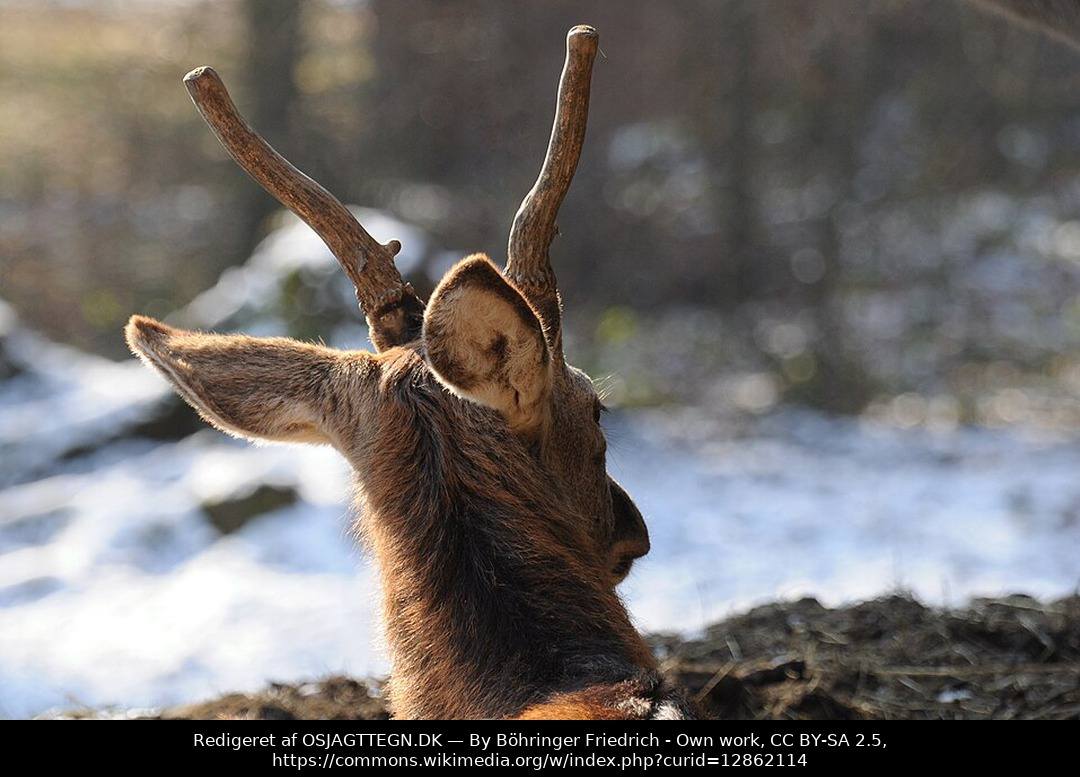
\includegraphics[width=\linewidth, height=7.2cm, keepaspectratio]{Billeder/Dyr/Pattedyr/hovdyr/kronvildt/kronspidshjort/kronspidshjort-01.JPG}
  \end{columns}
\end{frame}

% ========== KRONHIND ==========
\begin{frame}{%
  \begin{minipage}[c]{0.30\textwidth}
    Kronhind
  \end{minipage}%
  \hfill
  \begin{minipage}[c]{0.45\textwidth}
    \footnotesize
    \textbf{Jagttid:} 1.\ oktober -- 31.\ januar
  \end{minipage}%
  \hfill
  \begin{minipage}[c]{0.15\textwidth}
    \noindent\raggedleft
    
\includegraphics[width=0.5cm, height=0.5cm, keepaspectratio]{Billeder/Ikoner/star.png}%
    \hspace{0.2em}%
    
\includegraphics[width=0.5cm, height=0.5cm, keepaspectratio]{Billeder/Ikoner/star.png}%
    \hspace{0.2em}%
    
\includegraphics[width=0.5cm, height=0.5cm, keepaspectratio]{Billeder/Ikoner/star.png}
  \end{minipage}%
}
  \vspace{0.25em}
  \begin{columns}[T]
    \column{0.45\textwidth}
    \setlength{\parskip}{0.4em}
    \tiny
    \RaggedRight
    \textbf{\textit{Cervus elaphus}} – hunnen hos kronvildt. I andet leveår kaldes den smalhind, hvis den endnu ikke har fået kalv. Lever ofte i familiegruppe med kalv og andre hinder. \par
    \textbf{Udseende:}\\
    \quad – Intet gevir \\
    \quad – Langt snudeskaft \\
    \quad – Gult spejl der går op på ryggen \\
    \quad – Lange ører \par
    \textbf{Levesteder:} Store skovområder. Kræver meget ro. Nataktiv og opholder sig i tæt vegetation om dagen. \par
    \textbf{Føde:} Lyng, græs, lav, landbrugsafgrøder, skud fra buske/træer. \par
    %\textbf{Udbredelse:} Jylland og Sjælland. \par
    %\textbf{Parring/brunst:} September/oktober. \par
    \textbf{Forplantning:}\\
    \quad – \textbf{Kønsmoden:} 1 år \\
    \quad – \textbf{Mono/polygam:} Polygam \\
    \quad – \textbf{Bestandsomsætning:} Langsom \\
    \quad – \textbf{Kuld:} 1 kalv, sjældent 2 \par
    %\textbf{*Bemærk:} Mange lokale jagttider.
    \column{0.52\textwidth}
    \centering
    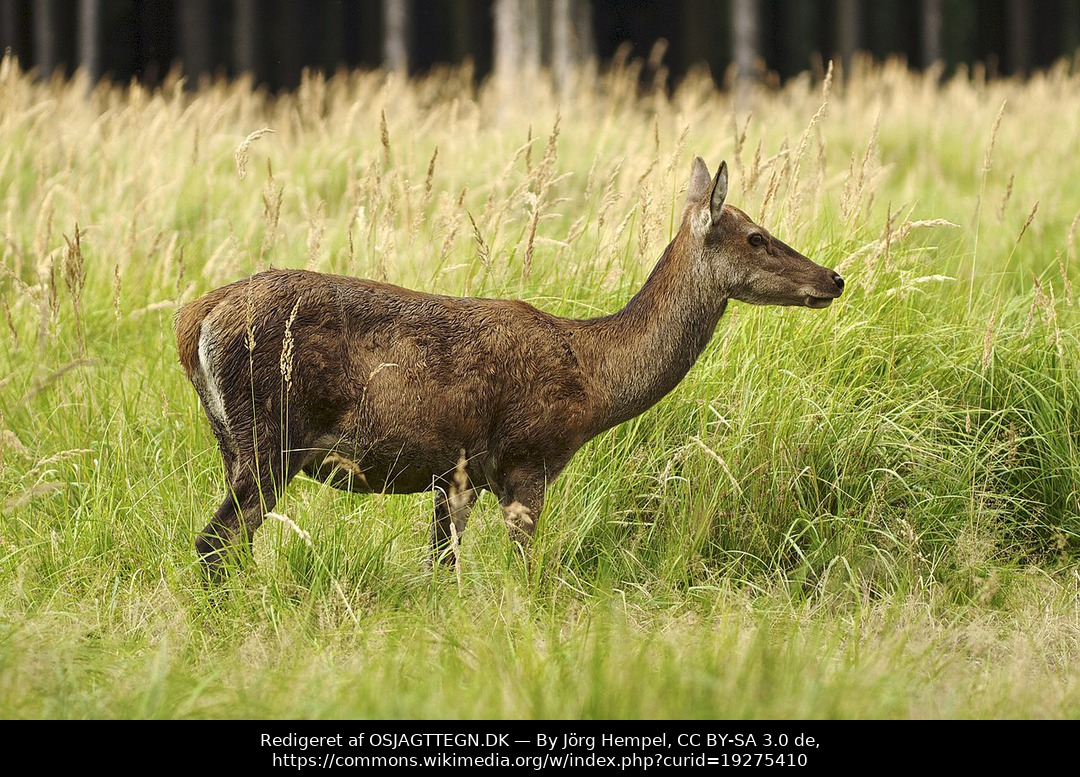
\includegraphics[width=\linewidth, height=7.2cm, keepaspectratio]{Billeder/Dyr/Pattedyr/hovdyr/kronvildt/kronhind/kronvildt-female-01.jpg}
  \end{columns}
\end{frame}

% ========== KRONKALV ==========
\begin{frame}{%
  \begin{minipage}[c]{0.30\textwidth}
    Kronkalv
  \end{minipage}%
  \hfill
  \begin{minipage}[c]{0.45\textwidth}
    \footnotesize
    \textbf{Jagttid:} 1.\ september -- 29.\ februar
  \end{minipage}%
  \hfill
  \begin{minipage}[c]{0.15\textwidth}
    \noindent\raggedleft
    
\includegraphics[width=0.5cm, height=0.5cm, keepaspectratio]{Billeder/Ikoner/star.png}%
    \hspace{0.2em}%
    
\includegraphics[width=0.5cm, height=0.5cm, keepaspectratio]{Billeder/Ikoner/star.png}%
    \hspace{0.2em}%
    
\includegraphics[width=0.5cm, height=0.5cm, keepaspectratio]{Billeder/Ikoner/star.png}
  \end{minipage}%
}
  \vspace{0.25em}
  \begin{columns}[T]
    \column{0.45\textwidth}
    \setlength{\parskip}{0.4em}
    \tiny
    \RaggedRight
    \textbf{\textit{Cervus elaphus}} – unge af kronvildt i sit første leveår. Lever typisk sammen med hinder og smalhinder i en familiegruppe eller rudel. \par
    \textbf{Udseende:}\\
    \quad – Mindre end hind og hjort \\
    \quad – Kortere hals og snudeskaft \\
    \quad – Intet gevir \\
    \quad – Gult spejl der går op på ryggen \\
    \quad – Kan have lyse pletter som helt lille \par
    %\textbf{Levesteder:} Store skovområder. Kræver meget ro. Nataktiv og opholder sig i tæt vegetation om dagen. \par
    %\textbf{Føde:} Lyng, græs, lav, landbrugsafgrøder, skud fra buske/træer. \par
    %\textbf{Udbredelse:} Jylland og Sjælland. \par
    %\textbf{Parring/brunst:} Født efter brunst i september/oktober. \par
    %\textbf{Forplantning:}\\
    %\quad – \textbf{Kønsmoden:} 1 år \\
    %\quad – \textbf{Mono/polygam:} Polygam \\
    %\quad – \textbf{Bestandsomsætning:} Langsom \\
    %\quad – \textbf{Kuld:} 1 kalv, sjældent 2 \par
    %\textbf{*Bemærk:} Mange lokale jagttider.
    \column{0.52\textwidth}
    \centering
    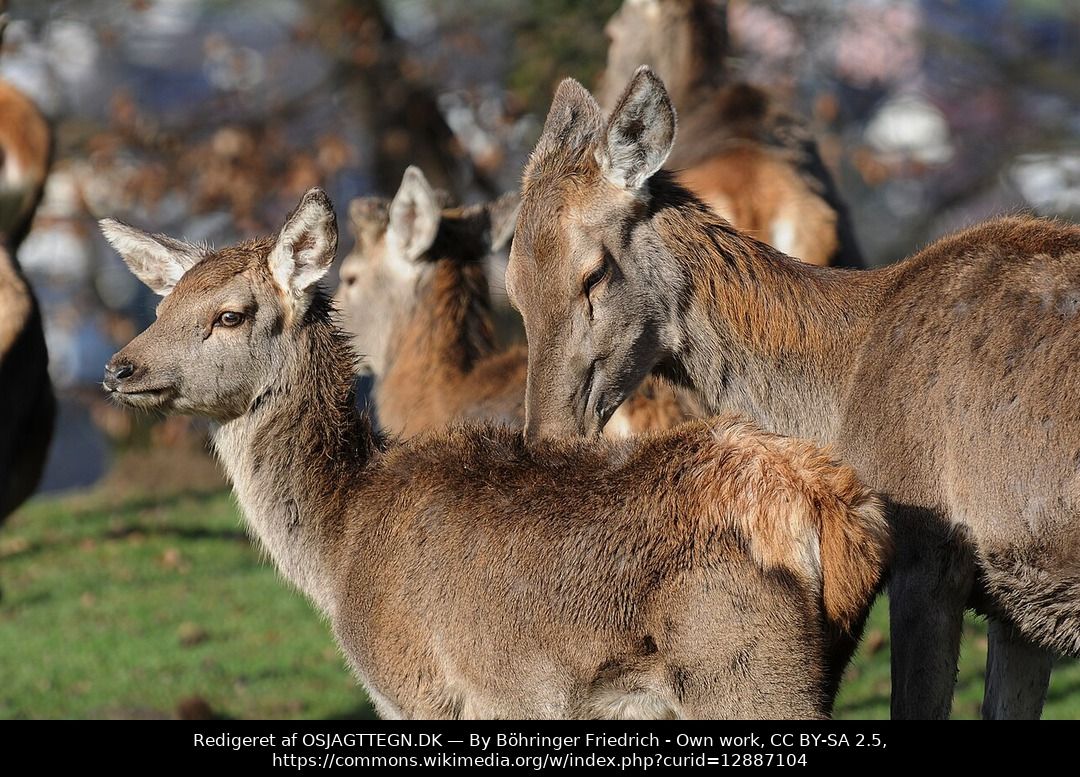
\includegraphics[width=\linewidth, height=7.2cm, keepaspectratio]{Billeder/Dyr/Pattedyr/hovdyr/kronvildt/kronkalv/kronvildt-female-05.jpeg}
  \end{columns}
\end{frame}

% ========== DÅHJORT ==========
\begin{frame}{%
  \begin{minipage}[c]{0.30\textwidth}
    Dåhjort
  \end{minipage}%
  \hfill
  \begin{minipage}[c]{0.45\textwidth}
    \footnotesize
    \textbf{Jagttid:} 1.\ september -- 31.\ januar
  \end{minipage}%
  \hfill
  \begin{minipage}[c]{0.15\textwidth}
    \noindent\raggedleft
    
\includegraphics[width=0.5cm, height=0.5cm, keepaspectratio]{Billeder/Ikoner/star.png}%
    \hspace{0.2em}%
    
\includegraphics[width=0.5cm, height=0.5cm, keepaspectratio]{Billeder/Ikoner/star.png}%
    \hspace{0.2em}%
    
\includegraphics[width=0.5cm, height=0.5cm, keepaspectratio]{Billeder/Ikoner/star.png}
  \end{minipage}%
}
  \vspace{0.25em}
  \begin{columns}[T]
    \column{0.45\textwidth}
    \setlength{\parskip}{0.4em}
    \tiny
    \RaggedRight
    \textbf{\textit{Dama dama}} – næststørste hjorteart i Danmark. Hannen kaldes dåhjort og kendes på det skovlede (plade) gevir. I andet leveår kaldes den dåspidshjort. \par
    \textbf{Udseende:}\\
    \quad – Kort snudeskaft \\
    \quad – Hvidt spejl (111) \\
    \quad – Mange farvevariationer med pletter \par
    \textbf{Levesteder:} Skov, hegn og åbne landskaber. \par
    \textbf{Føde:} Græsser, urter, olden og landbrugsafgrøder. \par
    \textbf{Udbredelse:} Hele landet. \par
    \textbf{Parring/brunst:} Oktober/november. \par
    \textbf{Forplantning:}\\
    \quad – \textbf{Kønsmoden:} 1 år \\
    \quad – \textbf{Mono/polygam:} Polygam \\
    \quad – \textbf{Bestandsomsætning:} Langsom \\
    \quad – \textbf{Kuld:} 1 kalv, sjældent 2 \par
    %\textbf{*Bemærk:} Mange lokale jagttider.
    \column{0.52\textwidth}
    \centering
    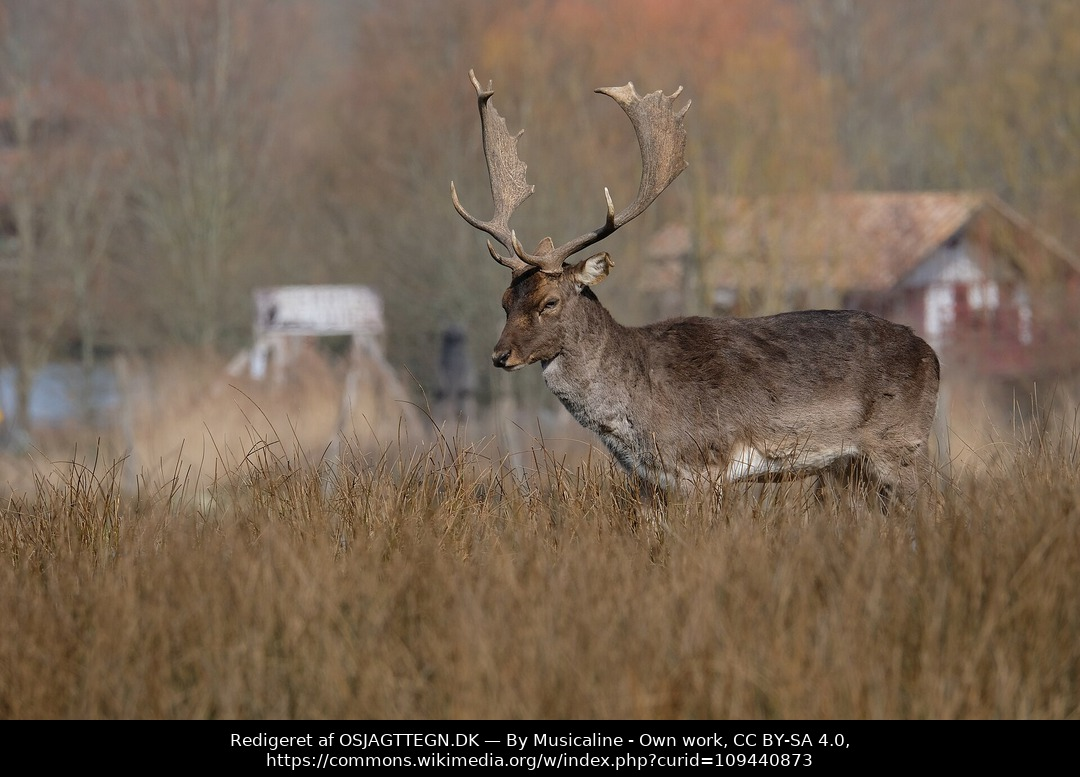
\includegraphics[width=\linewidth, height=7.2cm, keepaspectratio]{Billeder/Dyr/Pattedyr/hovdyr/dåvildt/daavildt-male-05.jpg}
  \end{columns}
\end{frame}

% ========== DÅSPIDSHJORT ==========
\begin{frame}{%
  \begin{minipage}[c]{0.30\textwidth}
    Dåspidshjort
  \end{minipage}%
  \hfill
  \begin{minipage}[c]{0.45\textwidth}
    \footnotesize
    \textbf{Jagttid:} 1.\ september -- 31.\ januar
  \end{minipage}%
  \hfill
  \begin{minipage}[c]{0.15\textwidth}
    \noindent\raggedleft
    
\includegraphics[width=0.5cm, height=0.5cm, keepaspectratio]{Billeder/Ikoner/star.png}%
    \hspace{0.2em}%
    
\includegraphics[width=0.5cm, height=0.5cm, keepaspectratio]{Billeder/Ikoner/star.png}%
    \hspace{0.2em}%
    
\includegraphics[width=0.5cm, height=0.5cm, keepaspectratio]{Billeder/Ikoner/star.png}
  \end{minipage}%
}
  \vspace{0.25em}
  \begin{columns}[T]
    \column{0.45\textwidth}
    \setlength{\parskip}{0.4em}
    \tiny
    \RaggedRight
    \textbf{\textit{Dama dama}} – dåhjort i sit andet leveår. Kaldes dåspidshjort, fordi geviret typisk kun består af to enkelte spidser. \par
    \textbf{Udseende:}\\
    \quad – To enkle gevirstænger uden skovle \\
    \quad – Kort snudeskaft \\
    \quad – Hvidt spejl (111) \\
    \quad – Mindre og slankere end ældre dåhjort \par
    \textbf{Levesteder:} Skov, hegn og åbne landskaber. \par
    \textbf{Føde:} Græsser, urter, olden og landbrugsafgrøder. \par
    \textbf{Udbredelse:} Hele landet. \par
    \textbf{Parring/brunst:} Oktober/november. \par
    \textbf{Forplantning:}\\
    \quad – \textbf{Kønsmoden:} 1 år \\
    \quad – \textbf{Mono/polygam:} Polygam \\
    \quad – \textbf{Bestandsomsætning:} Langsom \\
    \quad – \textbf{Kuld:} 1 kalv, sjældent 2 \par
    %\textbf{*Bemærk:} Mange lokale jagttider.
    \column{0.52\textwidth}
    \centering
    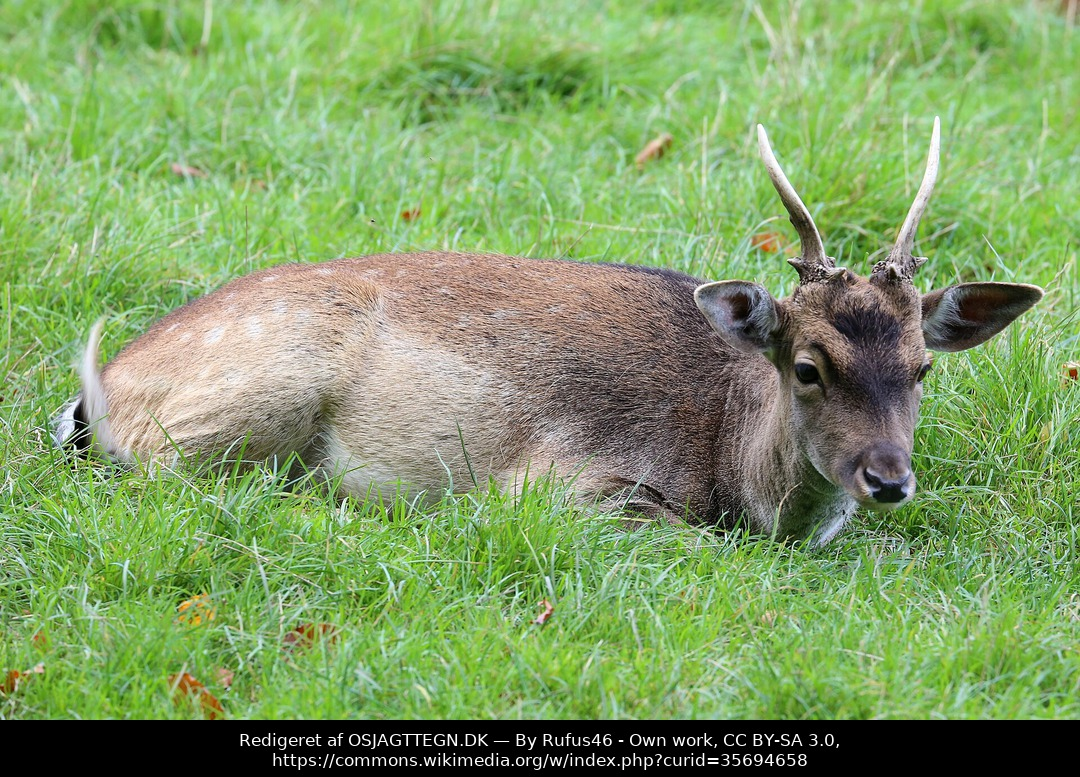
\includegraphics[width=\linewidth, height=7.2cm, keepaspectratio]{Billeder/Dyr/Pattedyr/hovdyr/dåvildt/dåspidshjort/daavildt-spidshjort-02.jpg}
  \end{columns}
\end{frame}

% ========== DÅ ==========
\begin{frame}{%
  \begin{minipage}[c]{0.30\textwidth}
    Då
  \end{minipage}%
  \hfill
  \begin{minipage}[c]{0.45\textwidth}
    \footnotesize
    \textbf{Jagttid:} 1.\ oktober -- 31.\ januar
  \end{minipage}%
  \hfill
  \begin{minipage}[c]{0.15\textwidth}
    \noindent\raggedleft
    
\includegraphics[width=0.5cm, height=0.5cm, keepaspectratio]{Billeder/Ikoner/star.png}%
    \hspace{0.2em}%
    
\includegraphics[width=0.5cm, height=0.5cm, keepaspectratio]{Billeder/Ikoner/star.png}%
    \hspace{0.2em}%
    
\includegraphics[width=0.5cm, height=0.5cm, keepaspectratio]{Billeder/Ikoner/star.png}
  \end{minipage}%
}
  \vspace{0.25em}
  \begin{columns}[T]
    \column{0.45\textwidth}
    \setlength{\parskip}{0.4em}
    \tiny
    \RaggedRight
    \textbf{\textit{Dama dama}} – hunnen hos dåvildt. I andet leveår kaldes den smaldå, hvis den endnu ikke har fået kalv. Då, smaldå og dåkalv lever ofte i familiegruppe. Flere dåer med afkom kaldes en rudel. \par
    \textbf{Udseende:}\\
    \quad – Intet gevir \\
    \quad – Kort snudeskaft \\
    \quad – Hvidt spejl (111) \\
    \quad – Mange farvevariationer med pletter \par
    \textbf{Levesteder:} Skov, hegn og åbne landskaber. \par
    \textbf{Føde:} Græsser, urter, olden og landbrugsafgrøder. \par
    \textbf{Udbredelse:} Hele landet. \par
    \textbf{Parring/brunst:} Oktober/november. \par
    \textbf{Forplantning:}\\
    \quad – \textbf{Kønsmoden:} 1 år \\
    \quad – \textbf{Mono/polygam:} Polygam \\
    \quad – \textbf{Bestandsomsætning:} Langsom \\
    \quad – \textbf{Kuld:} 1 kalv, sjældent 2 \par
    %\textbf{*Bemærk:} Mange lokale jagttider.
    \column{0.52\textwidth}
    \centering
    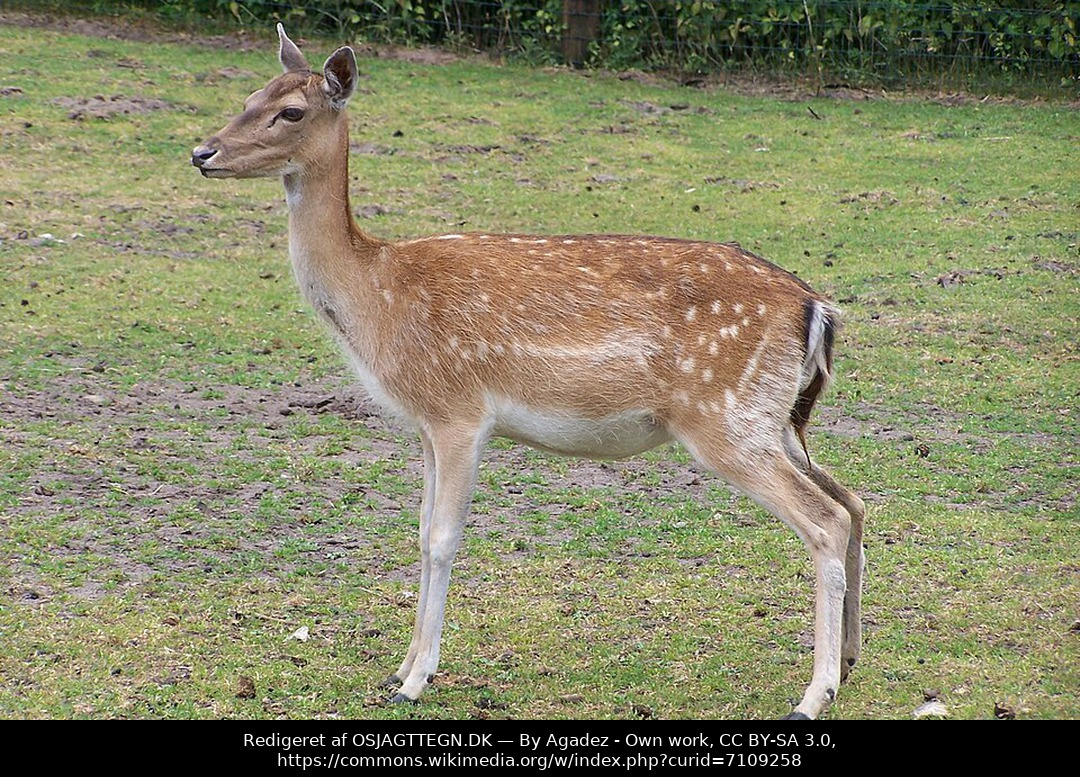
\includegraphics[width=\linewidth, height=7.2cm, keepaspectratio]{Billeder/Dyr/Pattedyr/hovdyr/dåvildt/daavildt-female-02.jpg}
  \end{columns}
\end{frame}

% ========== DÅKALV ==========
\begin{frame}{%
  \begin{minipage}[c]{0.30\textwidth}
    Dåkalv
  \end{minipage}%
  \hfill
  \begin{minipage}[c]{0.45\textwidth}
    \footnotesize
    \textbf{Jagttid:} 1.\ oktober -- 31.\ januar
  \end{minipage}%
  \hfill
  \begin{minipage}[c]{0.15\textwidth}
    \noindent\raggedleft
    
\includegraphics[width=0.5cm, height=0.5cm, keepaspectratio]{Billeder/Ikoner/star.png}%
    \hspace{0.2em}%
    
\includegraphics[width=0.5cm, height=0.5cm, keepaspectratio]{Billeder/Ikoner/star.png}%
    \hspace{0.2em}%
    
\includegraphics[width=0.5cm, height=0.5cm, keepaspectratio]{Billeder/Ikoner/star.png}
  \end{minipage}%
}
  \vspace{0.25em}
  \begin{columns}[T]
    \column{0.45\textwidth}
    \setlength{\parskip}{0.4em}
    \tiny
    \RaggedRight
    \textbf{\textit{Dama dama}} – unge af dåvildt i sit første leveår. Lever typisk sammen med dåen. \par
    \textbf{Udseende:}\\
    \quad – Mindre end då og dåhjort \\
    \quad – Intet gevir \\
    \quad – Hvidt spejl (111) \\
    \quad – Ofte tydeligt plettet, især som helt lille \par
    \textbf{Levesteder:} Skov, hegn og åbne landskaber. \par
    \textbf{Føde:} Græsser, urter, olden og landbrugsafgrøder. \par
    \textbf{Udbredelse:} Hele landet. \par
    \textbf{Parring/brunst:} Født efter brunst i oktober/november. \par
    \textbf{Forplantning:}\\
    \quad – \textbf{Kønsmoden:} 1 år \\
    \quad – \textbf{Mono/polygam:} Polygam \\
    \quad – \textbf{Bestandsomsætning:} Langsom \\
    \quad – \textbf{Kuld:} 1 kalv, sjældent 2 \par
    \column{0.52\textwidth}
    \centering
    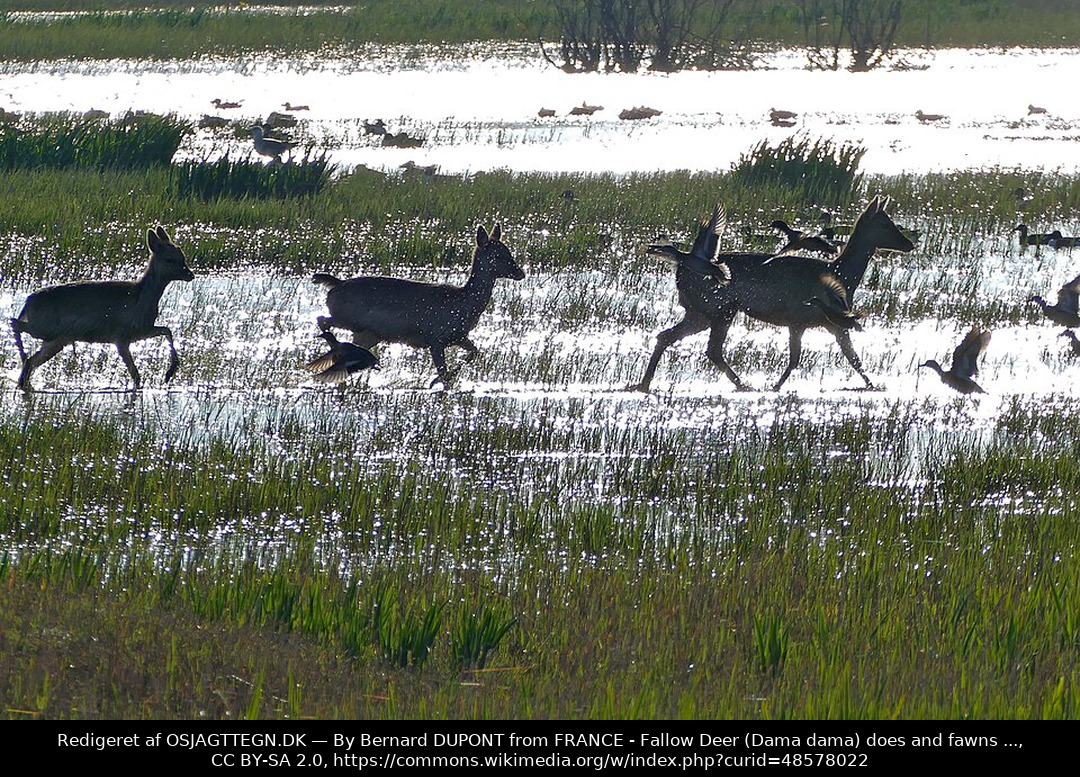
\includegraphics[width=\linewidth, height=7.2cm, keepaspectratio]{Billeder/Dyr/Pattedyr/hovdyr/dåvildt/daavildt-kalv-01.jpg}
  \end{columns}
\end{frame}

% ========== RÅBUK ==========
\begin{frame}{%
  \begin{minipage}[c]{0.30\textwidth}
    Råbuk
  \end{minipage}%
  \hfill
  \begin{minipage}[c]{0.45\textwidth}
    \footnotesize
    \textbf{Jagttid:} 16.\ maj -- 15.\ jul.\\
    samt 1.\ okt.--31.\ jan.
  \end{minipage}%
  \hfill
  \begin{minipage}[c]{0.15\textwidth}
    \noindent\raggedleft
    
\includegraphics[width=0.5cm, height=0.5cm, keepaspectratio]{Billeder/Ikoner/star.png}%
    \hspace{0.2em}%
    
\includegraphics[width=0.5cm, height=0.5cm, keepaspectratio]{Billeder/Ikoner/star.png}%
    \hspace{0.2em}%
    
\includegraphics[width=0.5cm, height=0.5cm, keepaspectratio]{Billeder/Ikoner/star.png}
  \end{minipage}%
}
  \vspace{0.25em}
  \begin{columns}[T]
    \column{0.45\textwidth}
    \setlength{\parskip}{0.4em}
    \tiny
    \RaggedRight
    \textbf{\textit{Capreolus capreolus}} – mindste hjorteart i Danmark. Hannen kaldes råbuk og kendes på det lille gevir. I andet leveår kaldes den spidsbuk. \par
    \textbf{Udseende:}\\
    \quad – Kort snudeskaft med sort plet \\
    \quad – Gulligt/hvidt spejl \\
    \quad – Rødbrun/grå \par
    \textbf{Levesteder:} Randzoner og nye skovarealer. Mest aktiv morgen og aften. \par
    \textbf{Føde:} Græsser, urter, knopper og skud fra buske. \par
    \textbf{Udbredelse:} Hele landet. \par
    \textbf{Yngleforhold:} Forlænget drægtighed. \par
    \textbf{Parring/brunst:} Slutningen af juli / starten af august. \par
    \textbf{Sygdomme:} Svælgbremser, pelslus
    \textbf{Forplantning:}\\
    \quad – \textbf{Kønsmoden:} 1 år \\
    \quad – \textbf{Mono/polygam:} Polygam \\
    \quad – \textbf{Bestandsomsætning:} Hurtig \\
    \quad – \textbf{Kuld:} 1--3 lam, oftest 2 \par
    %\textbf{*Bemærk:} Lokale jagttider kan forekomme.
    \column{0.52\textwidth}
    \centering
    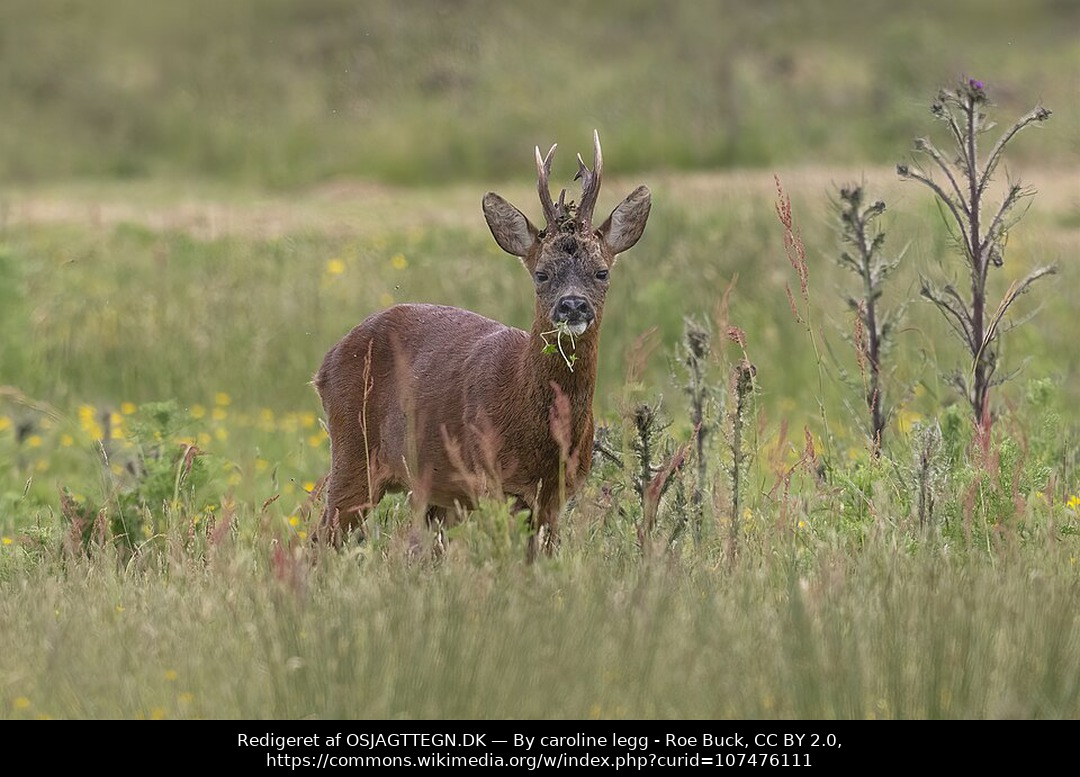
\includegraphics[width=\linewidth, height=7.2cm, keepaspectratio]{Billeder/Dyr/Pattedyr/hovdyr/råvildt/raavildt-male-10.jpg}
  \end{columns}
\end{frame}

% ========== RÅ OG RÅLAM ==========
\begin{frame}{%
  \begin{minipage}[c]{0.30\textwidth}
    Rå og rålam
  \end{minipage}%
  \hfill
  \begin{minipage}[c]{0.45\textwidth}
    \footnotesize
    \textbf{Jagttid:} 1.\ oktober -- 31.\ januar*
  \end{minipage}%
  \hfill
  \begin{minipage}[c]{0.15\textwidth}
    \noindent\raggedleft
    
\includegraphics[width=0.5cm, height=0.5cm, keepaspectratio]{Billeder/Ikoner/star.png}%
    \hspace{0.2em}%
    
\includegraphics[width=0.5cm, height=0.5cm, keepaspectratio]{Billeder/Ikoner/star.png}%
    \hspace{0.2em}%
    
\includegraphics[width=0.5cm, height=0.5cm, keepaspectratio]{Billeder/Ikoner/star.png}
  \end{minipage}%
}
  \vspace{0.25em}
  \begin{columns}[T]
    \column{0.45\textwidth}
    \setlength{\parskip}{0.4em}
    \tiny
    \RaggedRight
    \textbf{\textit{Capreolus capreolus}} – hunnen kaldes rå. En rå der har sat lam kaldes gammelrå. I andet leveår kaldes den smalrå. Ungen kaldes bukkelam eller rålam afhængigt af køn. \par
    \textbf{Udseende:}\\
    \quad – Kort snudeskaft med sort plet \\
    \quad – Gulligt/hvidt spejl \\
    \quad – Rødbrun/grå \par
    \textbf{Levesteder:} Randzoner og nye skovarealer. Mest aktiv morgen og aften. \par
    \textbf{Føde:} Græsser, urter, knopper og skud fra buske. \par
    \textbf{Udbredelse:} Hele landet. \par
    \textbf{Yngleforhold:} Forlænget drægtighed. \par
    \textbf{Parring/brunst:} Slutningen af juli / starten af august. \par
    \textbf{Forplantning:}\\
    \quad – \textbf{Kønsmoden:} 1 år \\
    \quad – \textbf{Mono/polygam:} Polygam \\
    \quad – \textbf{Bestandsomsætning:} Hurtig \\
    \quad – \textbf{Kuld:} 1--3 lam \par
    \textbf{*Bemærk:} Lokale jagttider kan forekomme.
    \column{0.52\textwidth}
    \centering
    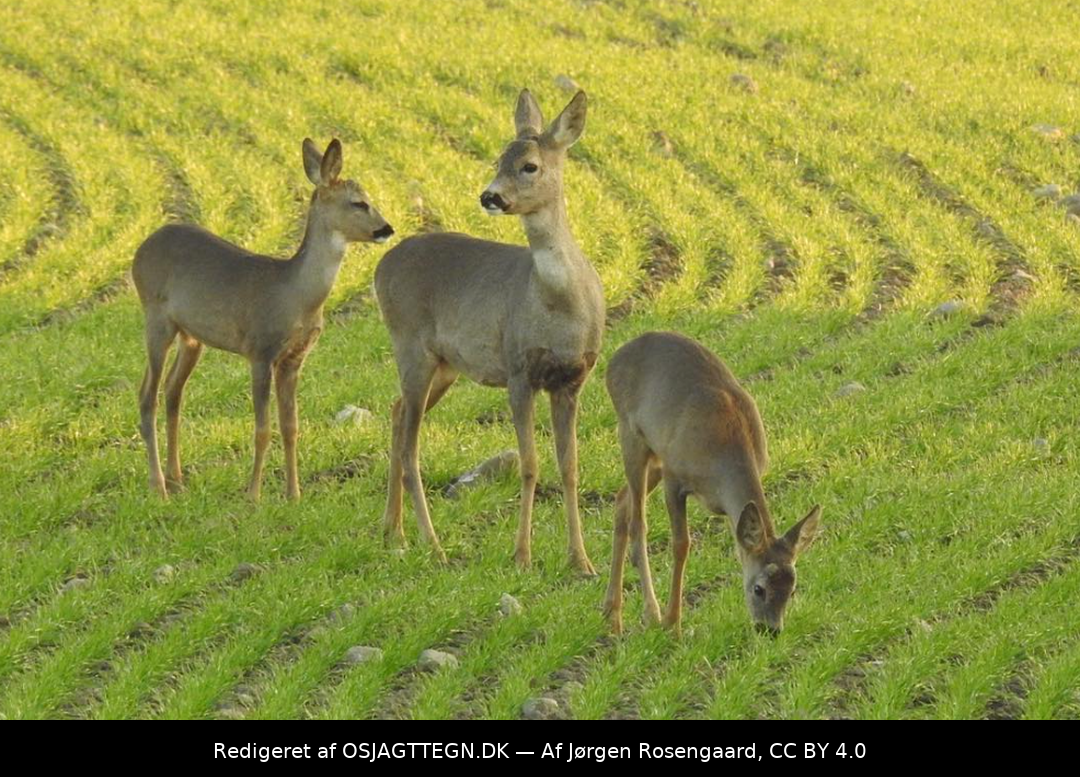
\includegraphics[width=\linewidth, height=7.2cm, keepaspectratio]{Billeder/Dyr/Pattedyr/hovdyr/råvildt/raavildt-family-01.png}
  \end{columns}
\end{frame}

% ========== SIKAHJORT ==========
\begin{frame}{%
  \begin{minipage}[c]{0.30\textwidth}
    Sikahjort
  \end{minipage}%
  \hfill
  \begin{minipage}[c]{0.45\textwidth}
    \footnotesize
    \textbf{Jagttid:} 1.\ september -- 31.\ januar
  \end{minipage}%
  \hfill
  \begin{minipage}[c]{0.15\textwidth}
    \noindent\raggedleft
    
\includegraphics[width=0.5cm, height=0.5cm, keepaspectratio]{Billeder/Ikoner/star.png}
  \end{minipage}%
}
  \vspace{0.25em}
  \begin{columns}[T]
    \column{0.45\textwidth}
    \setlength{\parskip}{0.4em}
    \tiny
    \RaggedRight
    \textbf{\textit{Cervus nippon}} – mindre hjorteart end kron- og dåvildt. Hannen kaldes sikahjort. \par
    \textbf{Udseende:}\\
    \quad – Hvidt spejl, men de sorte aftegninger fortsætter ned på bagbenene \\
    \quad – Ansigtsudtryk som med løftede øjenbryn \\
    \quad – Gevir uden skovle, typisk slankere end dåhjort \par
    \textbf{Levesteder:} Skov og skovbryn, især med tæt underskov. \par
    \textbf{Føde:} Græs, urter, skud og landbrugsafgrøder. \par
    \textbf{Udbredelse:} Især Djursland, men også andre steder i Danmark. \par
    \textbf{Parring/brunst:} Oktober. \par
    \textbf{Forplantning:}\\
    \quad – \textbf{Kønsmoden:} 1--2 år \\
    \quad – \textbf{Mono/polygam:} Polygam \\
    \quad – \textbf{Bestandsomsætning:} Langsom \\
    \quad – \textbf{Kuld:} 1 kalv
    \column{0.52\textwidth}
    \centering
    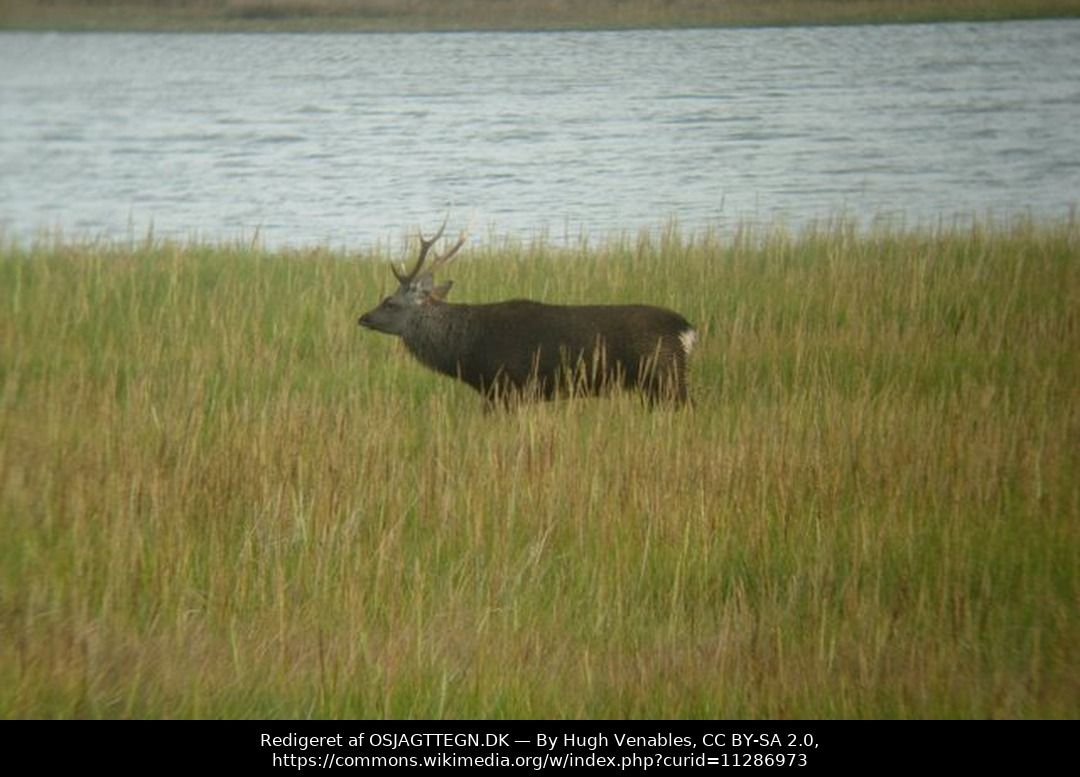
\includegraphics[width=\linewidth, height=7.2cm, keepaspectratio]{Billeder/Dyr/Pattedyr/hovdyr/sikavildt/sikavildt-male-06.jpg}
  \end{columns}
\end{frame}

% ========== SIKAHIND OG SIKAKALV ==========
\begin{frame}{%
  \begin{minipage}[c]{0.30\textwidth}
    Sikahind og sikakalv
  \end{minipage}%
  \hfill
  \begin{minipage}[c]{0.45\textwidth}
    \footnotesize
    \textbf{Jagttid:} 1.\ oktober -- 31.\ januar
  \end{minipage}%
  \hfill
  \begin{minipage}[c]{0.15\textwidth}
    \noindent\raggedleft
    
\includegraphics[width=0.5cm, height=0.5cm, keepaspectratio]{Billeder/Ikoner/star.png}
  \end{minipage}%
}
  \vspace{0.25em}
  \begin{columns}[T]
    \column{0.45\textwidth}
    \setlength{\parskip}{0.4em}
    \tiny
    \RaggedRight
    \textbf{\textit{Cervus nippon}} – hunnen kaldes sikahind. Ungen i første leveår kaldes sikakalv. Lever ofte sammen i mindre familiegrupper. \par
    \textbf{Udseende:}\\
    \quad – Intet gevir \\
    \quad – Hvidt spejl, hvor de sorte aftegninger fortsætter ned på bagbenene \\
    \quad – Ansigtsudtryk som med løftede øjenbryn \\
    \quad – Kalven er mindre og ofte tydeligere plettet \par
    \textbf{Levesteder:} Skov og skovbryn, især med tæt underskov. \par
    \textbf{Føde:} Græs, urter, skud og landbrugsafgrøder. \par
    \textbf{Udbredelse:} Især Djursland, men også andre steder i Danmark. \par
    \textbf{Parring/brunst:} Oktober. \par
    \textbf{Forplantning:}\\
    \quad – \textbf{Kønsmoden:} 1--2 år \\
    \quad – \textbf{Mono/polygam:} Polygam \\
    \quad – \textbf{Bestandsomsætning:} Langsom \\
    \quad – \textbf{Kuld:} 1 kalv
    \column{0.52\textwidth}
    \centering
    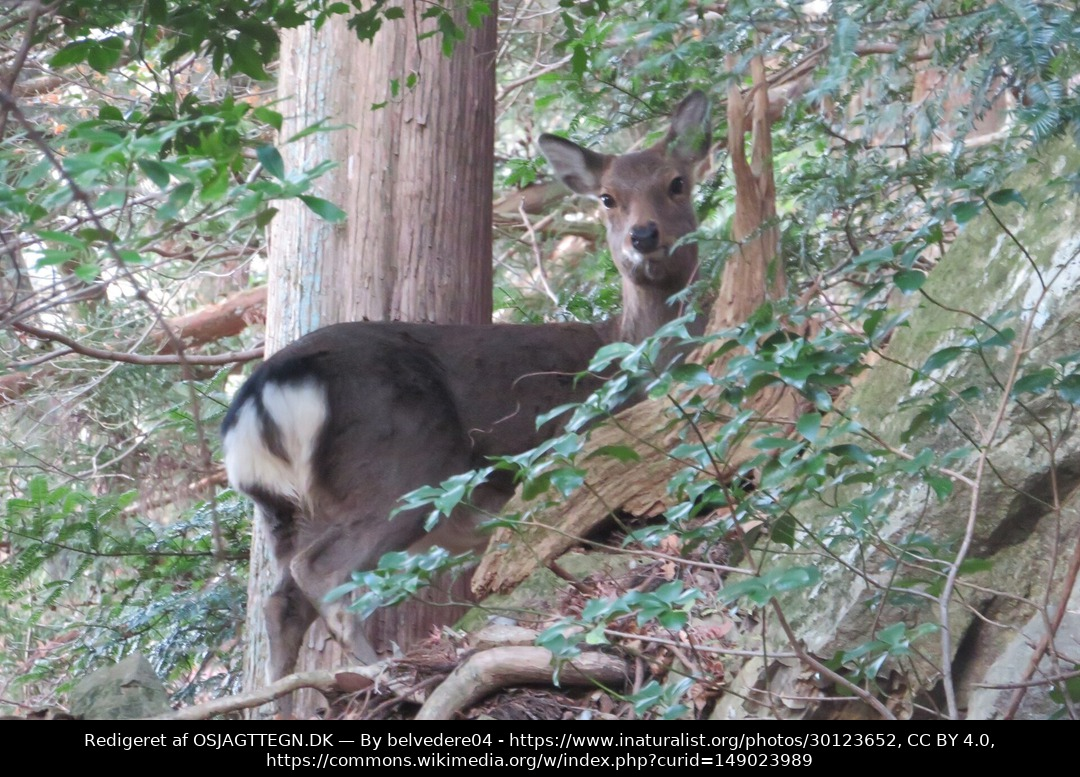
\includegraphics[width=\linewidth, height=7.2cm, keepaspectratio]{Billeder/Dyr/Pattedyr/hovdyr/sikavildt/sikavildt-female-01.jpg}
  \end{columns}
\end{frame}



\begin{frame}{Hjortevildtets spejl (rumpe)}
  \vspace{-0.3em}
  \centering
  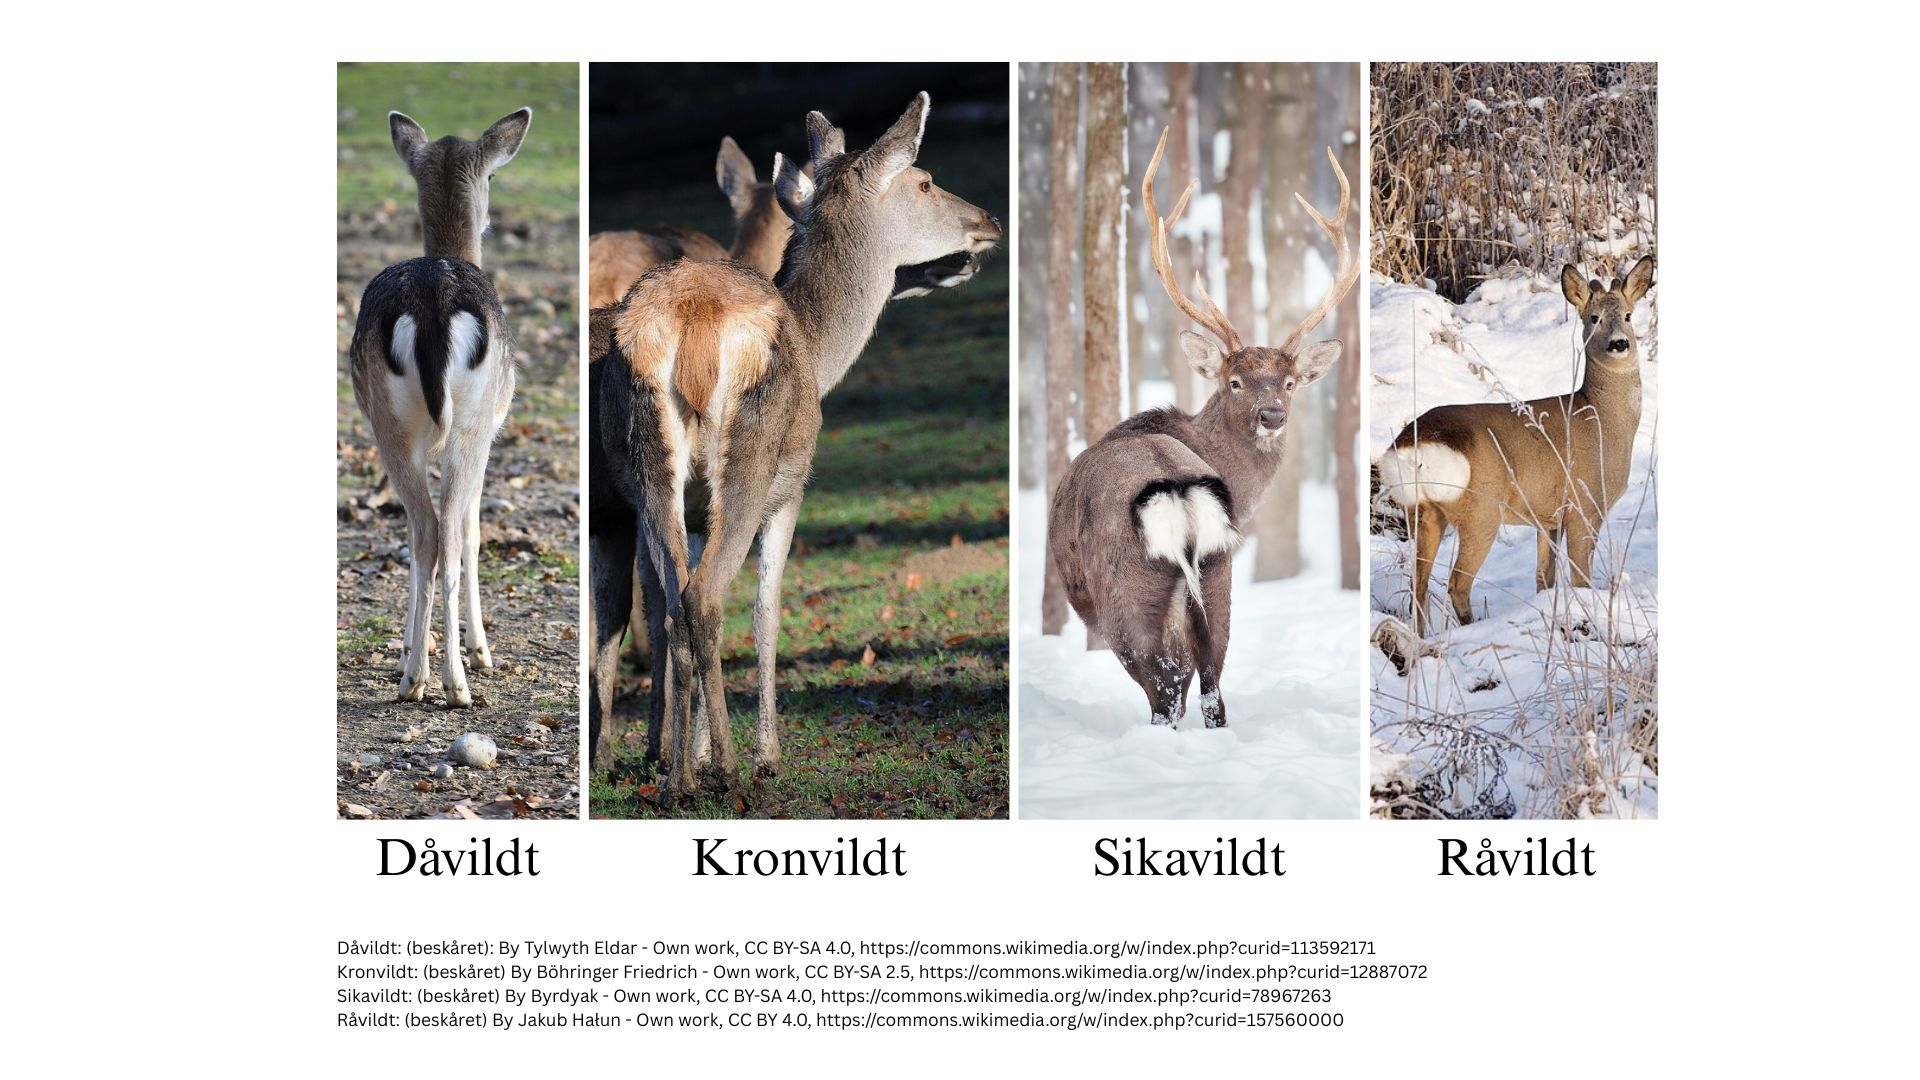
\includegraphics[width=0.95\textwidth, height=0.82\textheight, keepaspectratio]{Billeder/Dyr/Pattedyr/hovdyr/hjortevildtets_spejl.jpg}
\end{frame}

% ========== MUFLONVÆDDER ==========
\begin{frame}{%
  \begin{minipage}[c]{0.30\textwidth}
    Muflonvædder
  \end{minipage}%
  \hfill
  \begin{minipage}[c]{0.45\textwidth}
    \footnotesize
    \textbf{Jagttid:} 1.\ september -- 31.\ januar
  \end{minipage}%
  \hfill
  \begin{minipage}[c]{0.15\textwidth}
    \noindent\raggedleft
    
\includegraphics[width=0.5cm, height=0.5cm, keepaspectratio]{Billeder/Ikoner/star.png}
  \end{minipage}%
}
  \vspace{0.25em}
  \begin{columns}[T]
    \column{0.45\textwidth}
    \setlength{\parskip}{0.4em}
    \tiny
    \RaggedRight
    \textbf{\textit{Ovis musimon}} – vildt bjergfår indført til Danmark. Hannen kaldes vædder. \par
    \textbf{Udseende:}\\
    \quad – Store, bagudbøjede horn der ikke kastes, men vokser hele livet \\
    \quad – Rustrød til mørk pels med lyse saddelpletter på siden \\
    \quad – Kraftig krop og forholdsvis spinkle ben \par
    \textbf{Levesteder:} Åbne sletter, overdrev, hede og skovbryn. Trives dårligt i tæt skov. \par
    \textbf{Føde:} Græs og urter. Om vinteren også bark og stedsegrøn vegetation. \par
    \textbf{Udbredelse:} Enkelte småøer og udslip fra dyrehaver. \par
    %\textbf{Parring/brunst:} Efterår. \par
    %\textbf{Forplantning:}\\
    %\quad – \textbf{Kønsmoden:} Ca. 2--3 år \\
    %\quad – \textbf{Mono/polygam:} Polygam \\
    %\quad – \textbf{Bestandsomsætning:} Langsom \\
    %\quad – \textbf{Kuld:} 1 lam, sjældent 2
    \column{0.52\textwidth}
    \centering
    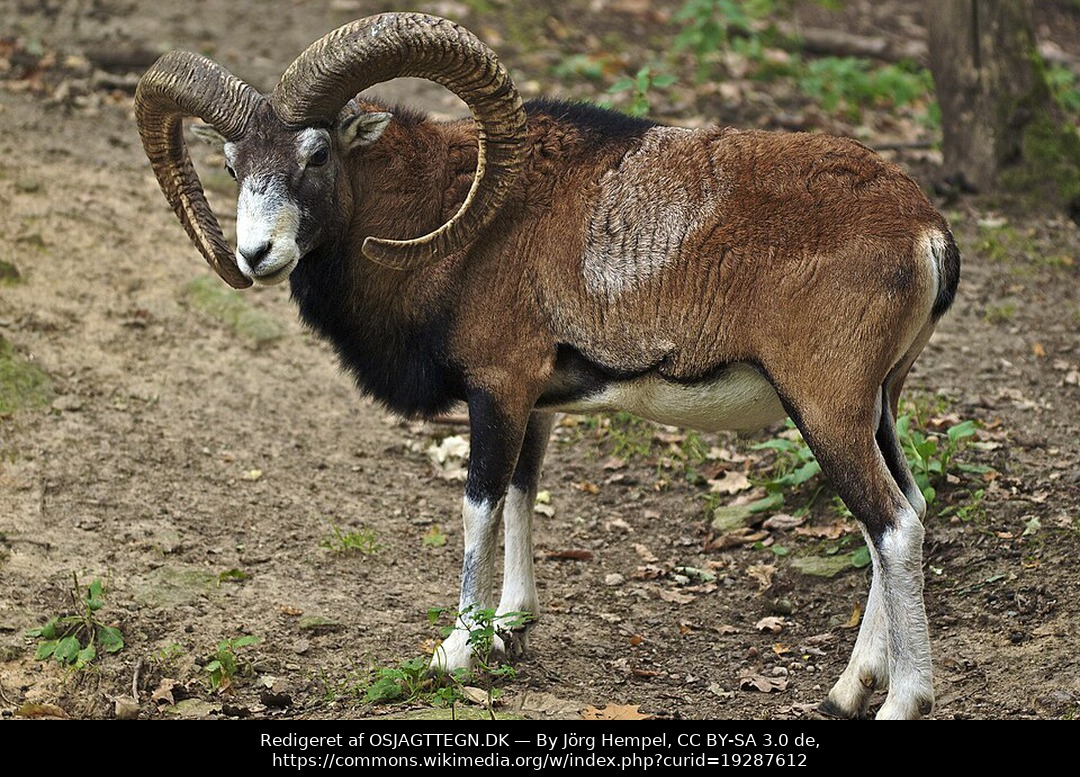
\includegraphics[width=\linewidth, height=7.2cm, keepaspectratio]{Billeder/Dyr/Pattedyr/hovdyr/muflon/muflon-male-01.jpg}
  \end{columns}
\end{frame}

% ========== MUFLONFÅR ==========
\begin{frame}{%
  \begin{minipage}[c]{0.30\textwidth}
    Muflonfår
  \end{minipage}%
  \hfill
  \begin{minipage}[c]{0.45\textwidth}
    \footnotesize
    \textbf{Jagttid:} 1.\ oktober -- 31.\ januar
  \end{minipage}%
  \hfill
  \begin{minipage}[c]{0.15\textwidth}
    \noindent\raggedleft
    
\includegraphics[width=0.5cm, height=0.5cm, keepaspectratio]{Billeder/Ikoner/star.png}
  \end{minipage}%
}
  \vspace{0.25em}
  \begin{columns}[T]
    \column{0.45\textwidth}
    \setlength{\parskip}{0.4em}
    \tiny
    \RaggedRight
    \textbf{\textit{Ovis musimon}} – hunnen hos muflon. Lever ofte i flok med lam og unge dyr. \par
    \textbf{Udseende:}\\
    \quad – Ingen eller kun korte horn \\
    \quad – Mindre end vædderen \\
    \quad – Rustrød til mørk pels, typisk uden de store lyse saddelpletter \\
    \quad – Kraftig krop og forholdsvis spinkle ben \par
    \textbf{Levesteder:} Åbne sletter, overdrev, hede og skovbryn. Trives dårligt i tæt skov. \par
    \textbf{Føde:} Græs og urter. Om vinteren også bark og stedsegrøn vegetation. \par
    \textbf{Udbredelse:} Enkelte småøer og udslip fra dyrehaver. \par
   % \textbf{Parring/brunst:} Efterår. \par
   % \textbf{Forplantning:}\\
    %\quad – \textbf{Kønsmoden:} Ca. 2 år \\
    %\quad – \textbf{Mono/polygam:} Polygam \\
    %\quad – \textbf{Bestandsomsætning:} Langsom \\
    %\quad – \textbf{Kuld:} 1 lam, sjældent 2
    \column{0.52\textwidth}
    \centering
    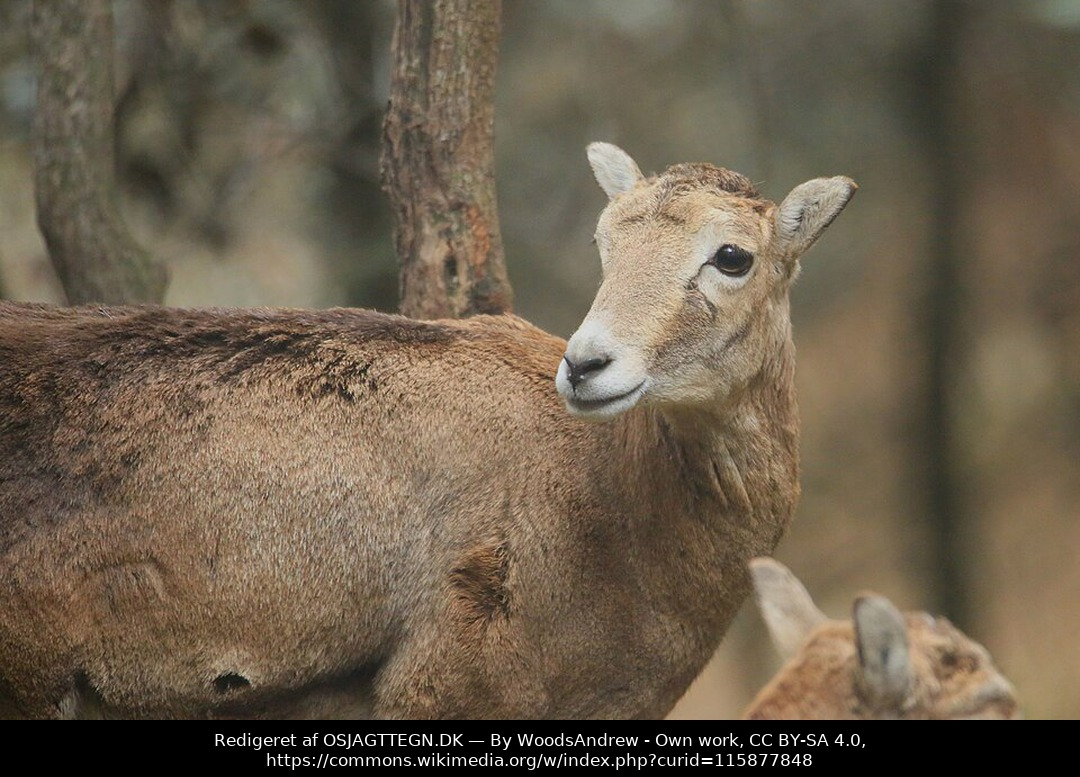
\includegraphics[width=\linewidth, height=7.2cm, keepaspectratio]{Billeder/Dyr/Pattedyr/hovdyr/muflon/muflon-female-01.jpg}
  \end{columns}
\end{frame}

% ========== VILDSVIN ==========
\begin{frame}{%
  \begin{minipage}[c]{0.30\textwidth}
    Vildsvin
  \end{minipage}%
  \hfill
  \begin{minipage}[c]{0.45\textwidth}
    \footnotesize
    \textbf{Jagttid:} Orne: 1.\ sep.--31.\ jan.\\
    So og gris: 1.\ okt.--31.\ jan.
  \end{minipage}%
  \hfill
  \begin{minipage}[c]{0.15\textwidth}
    \noindent\raggedleft
    
\includegraphics[width=0.5cm, height=0.5cm, keepaspectratio]{Billeder/Ikoner/star.png}%
    \hspace{0.2em}%
    
\includegraphics[width=0.5cm, height=0.5cm, keepaspectratio]{Billeder/Ikoner/star.png}
  \end{minipage}%
}
  \vspace{0.25em}
  \begin{columns}[T]
    \column{0.45\textwidth}
    \setlength{\parskip}{0.4em}
    \tiny
    \RaggedRight
    \textbf{\textit{Sus scrofa}} – langt, kegleformet hoved og kompakt krop med kraftig, børstet pels. Ornen har synlige hjørnetænder. \par
    \textbf{Benævnes:}\\
    \quad – Han: Orne \\
    \quad – Hun: So \\
    \quad – Unge: Gris \par
    \textbf{Udseende:}\\
    \quad – Ligner en gris \\
    \quad – Kraftig, strid pels \\
    \quad – Kompakt krop \par
    \textbf{Levesteder:} Findes i alle landskabstyper. Meget sky og nataktiv. \par
    \textbf{Føde:} Altædende, bl.a. planter, rødder, orme og ådsler. \par
    \textbf{Udbredelse:} Strejfende individer i Sydjylland. \par
    %\textbf{Forplantning:}\\
    %\quad – \textbf{Kønsmoden:} Ca. 1 år \\
    %\quad – \textbf{Mono/polygam:} Polygam \\
    %\quad – \textbf{Bestandsomsætning:} Hurtig \\
    %\quad – \textbf{Kuld:} 4--8 grise
    \column{0.52\textwidth}
    \centering
    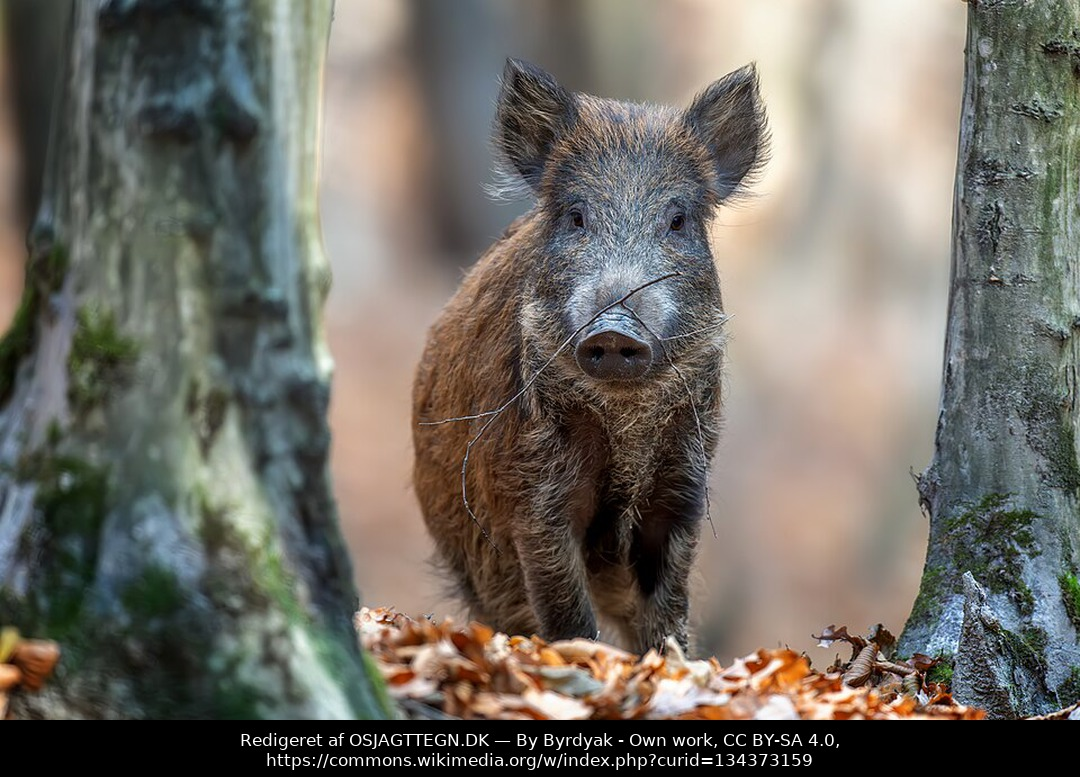
\includegraphics[width=\linewidth, height=7.2cm, keepaspectratio]{Billeder/Dyr/Pattedyr/hovdyr/vildsvin/vildsvin-01.jpg}
  \end{columns}
\end{frame}

\begin{frame}{Jagt på vildsvin}
  \vspace{-0.3em}
  \centering
  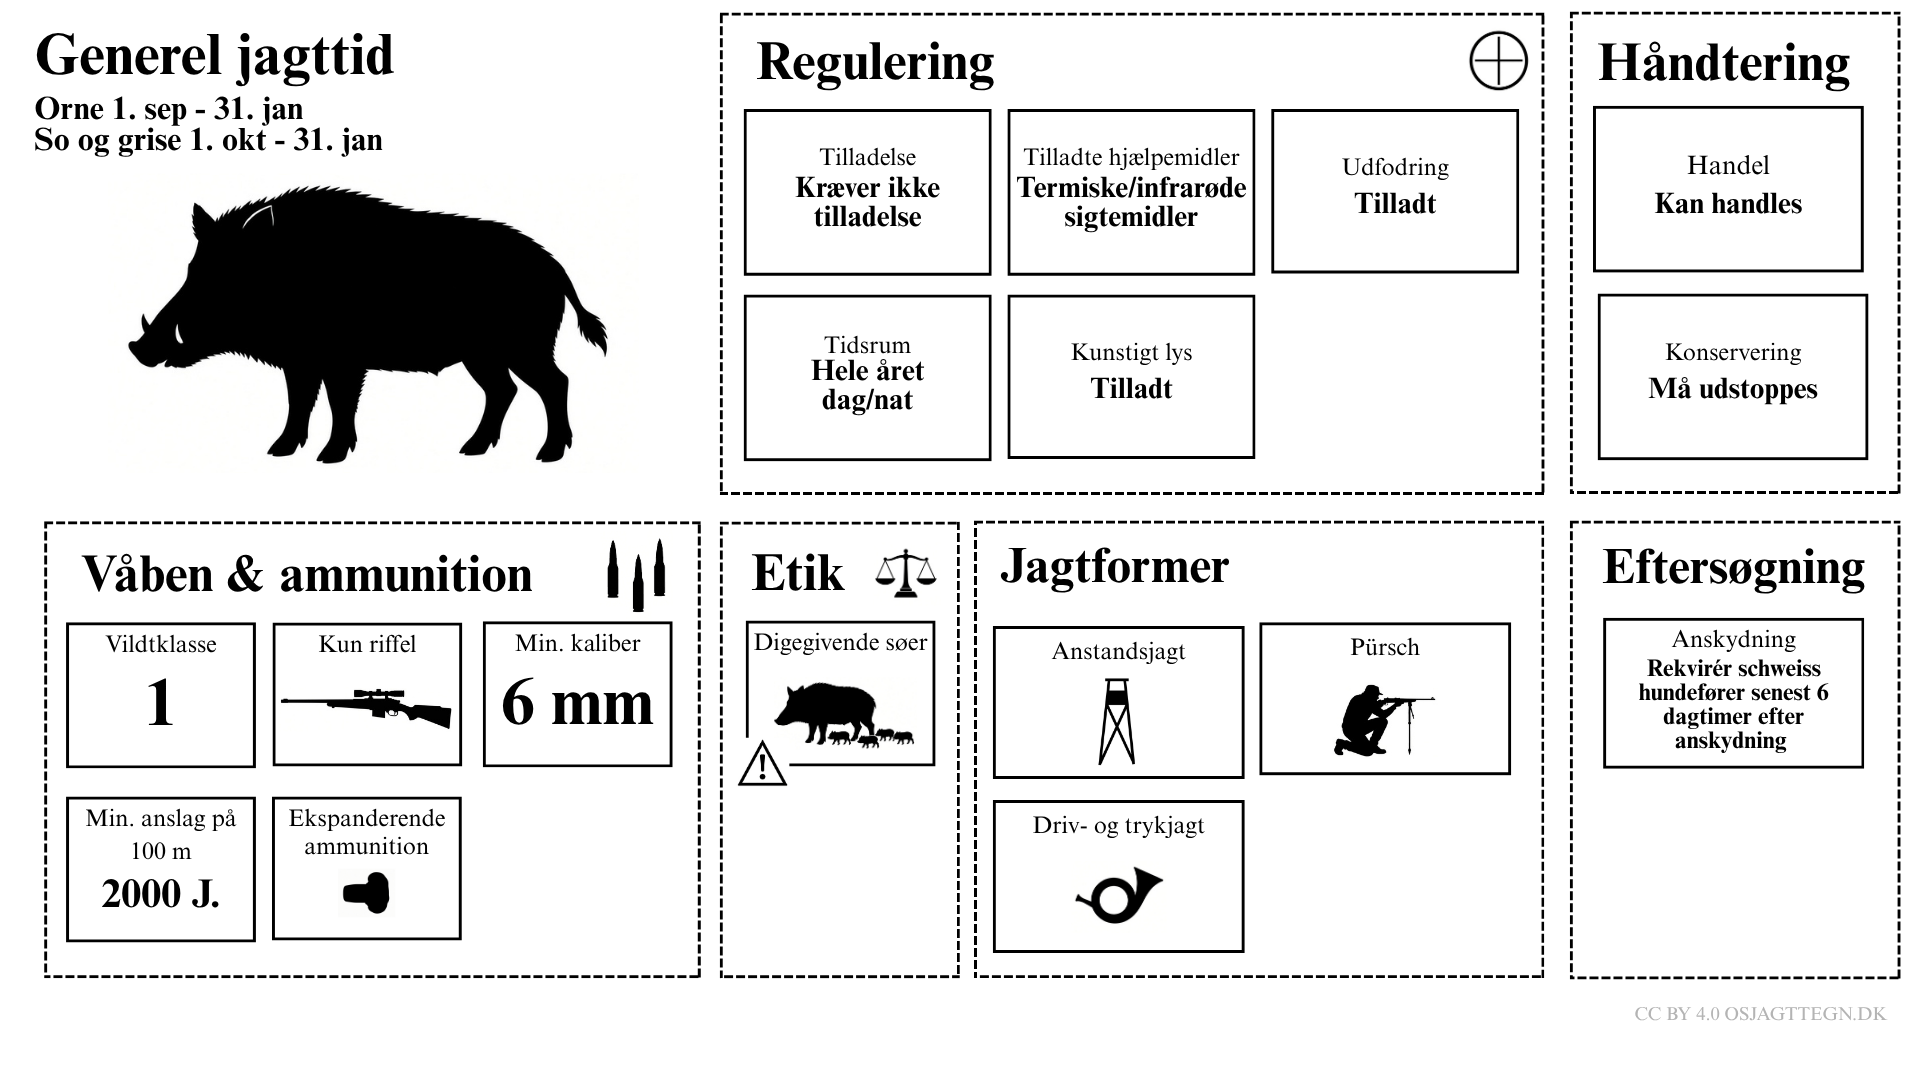
\includegraphics[width=0.95\textwidth, height=0.78\textheight, keepaspectratio]{Frames/Artsbestemmelse/Dyr/pattedyr/hovdyr/arter/vildsvin/info-vildsvin.png}
\end{frame}

%g\begin{frame}[plain]
\scriptsize
\vspace*{-1mm}

\newcommand{\ikon}[2][7mm]{%
  \IfFileExists{#2}{\includegraphics[height=#1]{#2}}{\rule{0pt}{#1}}%
}

\begin{columns}[T,onlytextwidth]
\begin{column}{0.25\textwidth}
\vspace*{4mm}
{\large\bfseries\color{myteal} Generel jagttid}\\[1mm]
{\scriptsize Orne 1.\ sep -- 31.\ jan\\
So og grise 1.\ okt -- 31.\ jan}\\[2mm]
\centering
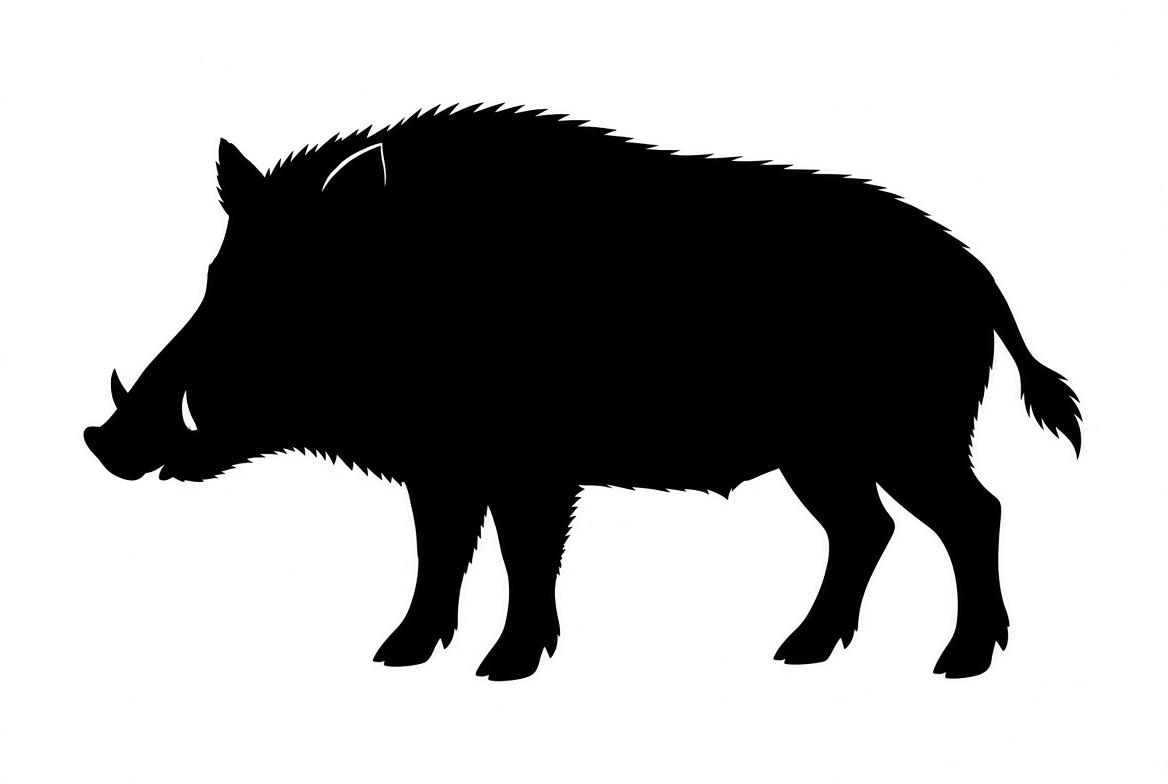
\includegraphics[width=0.95\linewidth,height=2.0cm,keepaspectratio]{Billeder/Ikoner/infografik/orne.jpg}
\end{column}

\begin{column}{0.49\textwidth}
\begin{tcolorbox}[gruppe, equal height group=toeraekke]
{\bfseries\color{myteal} Regulering}\\[0.6mm]
\begin{minipage}[t]{0.31\linewidth}
\begin{tcolorbox}[felt] Tilladelse\\ \textbf{Kræver ikke\\ tilladelse} \end{tcolorbox}
\end{minipage}\hfill
\begin{minipage}[t]{0.37\linewidth}
\begin{tcolorbox}[felt] Tilladte hjælpemidler\\ \textbf{Termiske/infr.\\ sigtemidler} \end{tcolorbox}
\end{minipage}\hfill
\begin{minipage}[t]{0.28\linewidth}
\begin{tcolorbox}[felt] Udfodring\\ \textbf{Tilladt} \end{tcolorbox}
\end{minipage}\\[0.8mm]
\begin{minipage}[t]{0.31\linewidth}
\begin{tcolorbox}[felt] Tidsrum\\ \textbf{Hele året\\ dag/nat} \end{tcolorbox}
\end{minipage}\hfill
\begin{minipage}[t]{0.37\linewidth}
\begin{tcolorbox}[felt] Kunstigt lys\\ \textbf{Tilladt} \end{tcolorbox}
\end{minipage}\hfill
\begin{minipage}[t]{0.28\linewidth}~\end{minipage}
\end{tcolorbox}
\end{column}

\begin{column}{0.24\textwidth}
\begin{tcolorbox}[gruppe, equal height group=toeraekke]
{\bfseries\color{myteal} Håndtering}\\[0.6mm]
\begin{tcolorbox}[feltfri] Handel\\ \textbf{Kan handles} \end{tcolorbox}\\[0.8mm]
\begin{tcolorbox}[feltfri] Konservering\\ \textbf{Må udstoppes} \end{tcolorbox}
\end{tcolorbox}
\end{column}
\end{columns}

\vspace{1mm}

\begin{columns}[T,onlytextwidth]
\begin{column}{0.34\textwidth}
\begin{tcolorbox}[gruppe, equal height group=bundraekke]
{\bfseries\color{myteal} Våben \& ammunition}\\[0.6mm]
\begin{minipage}[t]{0.30\linewidth}
\begin{tcolorbox}[felt] Vildtklasse\\ {\large\bfseries 1} \end{tcolorbox}
\end{minipage}\hfill
\begin{minipage}[t]{0.36\linewidth}
\begin{tcolorbox}[felt] Kun riffel\\[0.4mm]
\ikon[5mm]{Billeder/Ikoner/infografik/riffel.jpg}
\end{tcolorbox}
\end{minipage}\hfill
\begin{minipage}[t]{0.30\linewidth}
\begin{tcolorbox}[felt] Min.\ kaliber\\ \textbf{6 mm} \end{tcolorbox}
\end{minipage}\\[0.8mm]
\begin{minipage}[t]{0.48\linewidth}
\begin{tcolorbox}[felt] Min.\ anslag på 100 m\\ \textbf{2000 J.} \end{tcolorbox}
\end{minipage}\hfill
\begin{minipage}[t]{0.48\linewidth}
\begin{tcolorbox}[felt] Ekspanderende ammunition\\[0.4mm]
\ikon[5mm]{Billeder/Ikoner/infografik/ekspanderende_projektil.jpg}
\end{tcolorbox}
\end{minipage}
\end{tcolorbox}
\end{column}

\begin{column}{0.15\textwidth}
\begin{tcolorbox}[gruppe, equal height group=bundraekke]
{\bfseries\color{myteal} Etik}\\[0.6mm]
\begin{tcolorbox}[feltfri]
Digegivende søer\\[0.4mm]
\ikon[7mm]{Billeder/Ikoner/infografik/so_med_grise.jpg}\\[0.2mm]
\ikon[3mm]{Billeder/Ikoner/infografik/vær_opmærksom.jpg}
\end{tcolorbox}
\end{tcolorbox}
\end{column}

\begin{column}{0.28\textwidth}
\begin{tcolorbox}[gruppe, equal height group=bundraekke]
{\bfseries\color{myteal} Jagtformer}\\[0.6mm]
\begin{minipage}[t]{0.48\linewidth}
\begin{tcolorbox}[felt] Anstand\\[0.4mm]
\ikon[6mm]{Billeder/Ikoner/infografik/jagttårn.png}
\end{tcolorbox}
\end{minipage}\hfill
\begin{minipage}[t]{0.48\linewidth}
\begin{tcolorbox}[felt] Pürsch\\[0.4mm]
\ikon[6mm]{Billeder/Ikoner/infografik/purschjagt.jpg}
\end{tcolorbox}
\end{minipage}\\[0.8mm]
\begin{minipage}[t]{0.48\linewidth}
\begin{tcolorbox}[felt] Driv/trykjagt\\[0.4mm]
\ikon[6mm]{Billeder/Ikoner/infografik/drivjagt.jpg}
\end{tcolorbox}
\end{minipage}
\end{tcolorbox}
\end{column}

\begin{column}{0.21\textwidth}
\begin{tcolorbox}[gruppe, equal height group=bundraekke]
{\bfseries\color{myteal} Eftersøgning}\\[0.6mm]
\begin{tcolorbox}[feltfri]
Anskydning\\
\textbf{Rekvirér schweiss}\\
senest \textbf{6 dagtimer}\\
efter anskydning
\end{tcolorbox}
\end{tcolorbox}
\end{column}
\end{columns}

\vspace{1mm}
\hfill{\tiny\color{gray} CC BY 4.0 \href{https://osjagttegn.dk}{OSJAGTTEGN.DK}}
\end{frame}

\begin{frame}{Benævnelser for hovdyr}

    \small

    \begin{table}
    \centering
    \resizebox{\textwidth}{!}{
        \begin{tabular}{|l|c|c|c|c|c|c|c|}
        \hline
        \textbf{Benævnelser} & \textbf{Han} & \textbf{Hun} & \textbf{2. års han} & \textbf{2. års hun} & \textbf{Unge han} & \textbf{Unge hun} & \textbf{Flok} \\
        \hline
        \textbf{Kronvildt} & \underline{Kronhjort} & \underline{Kronhind} & \underline{Spidskronhjort} & \underline{Smalkronhind} & \multicolumn{2}{c|}{\underline{Kronkalv}} & \underline{Rudel} \\ \hline
        \textbf{Dåvildt} & \underline{Dåhjort} & \underline{Då} & \underline{Spidsdåhjort} & \underline{Smaldå} & \multicolumn{2}{c|}{\underline{Dåkalv}} & \underline{Rudel} \\ \hline
        \textbf{Sikavildt} & \underline{Sikahjort} & \underline{Sikahind} & \underline{Spidssikahjort} & \underline{Smalsikahind} & \multicolumn{2}{c|}{\underline{Sikakalv}} & \underline{Rudel} \\ \hline
        \textbf{Råvildt} & \underline{Råbuk} & \underline{Rå} & \underline{Spidsbuk} & \underline{Smalrå} & \underline{Bukkelam} & \underline{Rålam} & \underline{Spring} \\ \hline
        \textbf{Vildsvin} & \underline{Orne} \textit{(Korrekt: Keiler)} & \underline{So} & \multicolumn{2}{c|}{\textit{Overløber}} & \multicolumn{2}{c|}{\underline{Gris} \textit{(Korrekt: Grisling)}} & \textit{Rotte} \\ \hline
        \textbf{Muflon} & \underline{Vædder} & \underline{Får} & \textit{Årling} & \textit{Gimmer} & \multicolumn{2}{c|}{\underline{Lam}} & \textit{Hjord} \\ \hline
        \textit{\textbf{Elg}} & \textit{Tyr} & \textit{Ko} & \textit{Ungtyr} & \textit{Kvie} & \textit{Tyrekalv} & \textit{Kalv} & --- \\
        \hline
        \end{tabular}
    }
    \end{table}

    \vspace{0.4em}
    \tiny
    \textit{Note: Arter og benævnelser i \textit{kursiv} er ikke pensum}

\end{frame}

\begin{frame}
  \vspace{1.8em}
  \begin{center}
    \begin{minipage}{0.22\textwidth}
      \centering
      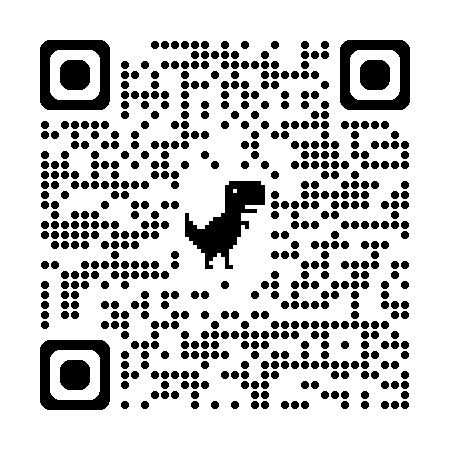
\includegraphics[width=\linewidth]{Billeder/Dyr/Pattedyr/hovdyr/hovdyr_qr.png}
    \end{minipage}%
    \hspace{0.8em}%
    \begin{minipage}{0.62\textwidth}
      \raggedright
      \Large
      \textbf{Træning i artsbestemmelse af hovdyr}\\[0.35em]
      {\large https://osjagttegn.dk/hovdyr}
    \end{minipage}
  \end{center}
\end{frame}

